\section{Symbolic Dynamic Programming Cores}
\label{SymbolicDPCores}

In this section we introduce our main technical contribution. More specifically, we introduce the notion of symbolic dynamic programming core, a formalism that can be used to define dynamic programming algorithms operating on $k$-instructive tree decompositions where sets of partial solutions asociated with each node are represented implicitly, using OBDDs. 

A {\em symbolic dynamic programming core} (SDP-core) operating on $k$-instructive tree decompositions is a record $\sdpcore[k]$ consisting of the following components, where $\activelabelu,\activelabelv \in [k+1]$, and 
$\activelabelu\neq \activelabelv$. 

\begin{itemize}
    \item $\symbleaf$ is an OBDD $\ODD\in \allodds(\{0,1\})$. 
    \item $\symbintrovertex{\nodeu}:2^{[k]}\times  
    \allodds(\{0,1\})\rightarrow \allodds(\{0,1\})$;
    \item $\symbintroedge{\nodeu}{\activelabelv}:2^{[k]}\times\allodds(\{0,1\})\rightarrow \allodds(\{0,1\})$;
    \item $\symbforgetvertex{\nodeu}:2^{[k]}\times \allodds(\{0,1\})\rightarrow \allodds(\{0,1\})$;
    \item $\symbjoin:2^{[k]}\times \allodds(\{0,1\})\times 
    \allodds(\{0,1\})
    \rightarrow 
    \allodds(\{0,1\})$.
    \item $\final:\{0,1\}^*\rightarrow \{0,1\}$. 
    \item $\inv:2^{\{0,1\}^*}\rightarrow \N$. 
\end{itemize}


Intuitively, a symbolic DP-core processes a $k$-instructive tree decomposition from the leaves towards the root, and assigns to each node of the decomposition an OBDD representing a set of strings enconding partial solutions of a given combinatorial problem. The SDP-core assigns to each leaf node of the decomposition the OBDD $\symbleaf$. Suppose that $\nodep$ is a node with a single child $p'$, and let $\ODD(\nodep')$ be the OBDD associated with $\nodep'$. Then the SDP assigns to $\nodep$ the OBDD 
$\symbintrovertex{\nodeu}(b(\nodep'),\ODD)$, if $u$ is introduced at $\nodep$, the OBDD 
$\symbforgetvertex{\nodeu}(b(\nodep'),\ODD)$, if $u$ is forgotten at $\nodep$, and 
$\symbintroedge{\activelabelu}{\activelabelv}(b(\nodep'),\ODD)$ if edge $\{\activelabelu,\activelabelv\}$ is introduced at $\nodep$. Finally, if $\nodep$ is a join node with children $\nodep'$ and $\nodep''$, then the SDP assigns to $\nodep$ the OBDD 
$\symbjoin(\ODD(\nodep'),\ODD(\nodep''))$. 

The SDP-core $\sdpcore$ accepts a $k$-instructive tree decomposition  $\treedec$ if the language $\Lang(\ODD(\rootfunction{\treedec}))$ of the OBDD associated with the root node of $\treedec$ contains a final witness, 
that is, a string $w$ such that $\final(w)=1$. The SDP-core $\sdpcore$ is {\em coherent} if for 
each graph $\graph$ of treewidth at most $k$, and each two $k$-instructive tree 
decomposition $\treedec,\treedec'$ of $\graph$, $\sdpcore$ accepts $\treedec$ if and only if 
it accepts $\treedec'$. We say that a coherent SDP-core $\sdpcore$ computes a graph invariant 
$\invariant$ if $\inv(\Lang(\ODD(\rootfunction{\treedec}))) = \invariant(\graph)$ for each $k$-instructive tree decomposition $\treedec$ of $\graph$. 


\section{Symbolic Vertex Cover}\label{Symbolic Vertex Cover (sketch)}

In this section, we define a concrete example of a symbolic dynamic programming core for the {\sc Vertex Cover} problem. We start by defining a local witness for this problem, which intuitively will serve as an encoding of a partial solution of the problem. 
If $\nodep$ is a node of a $k$-instructive tree decomposition whose set of active labels is $\activelabels$, then a local witness at this node is a string of the form $s\cdot t$ where $s$ is a binary string of length $|\activelabels|$ representing a subset of active labels, while $t$ is (the binary encoding of) a number representing the size of the solution. We may refer to $s$ as the \textit{string component} and number $t$ as the \textit{size component} of the witness. The subset represented by $s$ depends on the set of labels $\activelabels \subseteq [k+1]$, that are active at a given node of the tree decomposition. More specifically, let $l_1 < ... < l_{|s|}, l_i \in \activelabels$ be the active labels at a given node $\nodep$. Then the set represented by $s$ is $Active(s) = \{l_j \;:\; s_j=1\}$. For instance, let
$\activelabels = \{2,4,5\}$ be the set of active labels at node $p$, then $s=101$ represents the set $\{2,5\}$ while $s'=011$ represents the set $\{4,5\}$. 

\begin{comment}
In this section, we introduce the main technical component of our symbolic algorithm. In particular, we will show that if we are given a subset $b \subseteq [k+1]$ and an OBDD $\ODD$ representing a set of partial solutions $\Lang(\ODD)$, then for each operation $\mathrm{op}\in\{\introvertex{\activelabelu},\introedge{\activelabelu}{\activelabelv},\\ \forgetvertex{\activelabelu},\join\}$ in the Vertex Cover DP-core, one can construct an OBDD $\mathrm{op}(b, \ODD)$ whose language is 

\begin{equation}
\Lang(\mathrm{op}(b, \ODD)) = \mathrm{op}(b,\Lang(\ODD))
\end{equation}

One important aspect of our construction is that the OBDD $\mathrm{op}(\ODD)$ can be constructed in polynomial time on the size of $\ODD$. It is worth noting that a naive construction, where one explicitly enumerates the strings in $\Lang(\ODD)$, applies the operation $\mathrm{op}$ according to Definition \ref{VCDP-core} and then minimizes the resulting OBDD would take time exponential on the number of layers of $\ODD$. 
\end{comment}

In the next subsections, we define the operations performed on OBDDs representing sets of witnesses at each node of a $k$-instructive tree decomposition for a graph $G = (V,E)$ when solving the {\sc Vertex Cover} problem.
In particular, at node $p$ of our tree decomposition with active labels $b\subseteq [k+1]$, a set of witnesses will be represented by an ODD $D = B_1B_2\ldots B_{|\activelabels|+1}$ of length $|\activelabels|+1$, where the first $|b|$ layers read the string component of a witness and layer $|\activelabels|+1$ reads the size component of a witness. Each label $u\in \activelabels$ corresponds to a single layer of the OBDD. We denote this layer by $B_{\activelabels[\activelabelu]}$. For clarity, in the final layer, the size component is represented as a number $t\in [|V|]$. However, this final layer can be easily replaced by $\log |V|$ layers that read the binary encoding of $t$. Therefore, for simplicity, throughout this section we will refer to these ODDs simply as OBDDs. 
%In particular, when solving {\sc Vertex Cover} on a graph $G$, our OBDDs will have a varying number of layers depending on the current number of active labels.
To provide an intuition of the meaning of the operations we perform, we will refer to the operations performed in the standard DP-core for the {\sc Vertex Cover} problem. For completeness, a full definition of this DP-core is provided in Appendix \ref{subsection:VC}.

\subsection{Leaf Nodes}

In the standard DP-core for {\sc Vertex Cover} (Appendix \ref{subsection:VC}, Definition \ref{VCDP-core}), the singleton $\{0\}$ is assigned to each leaf of the tree decomposition. Here, $0$ is an encoding of an empty set of vertices, since the graph associated with the leaf is the empty graph. Consequently, we define the corresponding symbolic component $\symbleaf$, as the OBDD $\ODD = \B$ representing the set of partial solutions for {\sc Vertex Cover} at leaf nodes. The OBDD $\ODD$ comprises a single layer accepting only value $0$, which is the size of the empty set of vertices. All other numbers in $\dbset{|V|}$ are rejected by the OBDD. This OBDD is shown in Figure \ref{fig:Leaf} below:

\begin{figure}[h]
    \centering
    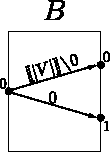
\includegraphics[width=0.25\linewidth]{IJCAI25/Figures/OBDDsResized/LeafResized.pdf}
    \caption{\symbleaf}
    \label{fig:Leaf}
\end{figure}

We define layer $B$ explicitly as consisting of a single transition from the initial state to the accept state labeled with value $0$, while all other transitions labeled with a value from $\dbset{|V|} \setminus \{0\}$ lead to the reject state: $B = \{(0,0,\accept)\} \cup \{(0,l,\reject): l \in \dbset{|V|}\}$.

\subsection{Intro Vertex}

In the standard DP-core for {\sc Vertex Cover} (Appendix \ref{subsection:VC}, Definition \ref{VCDP-core}), if $w$ is a local witness corresponding to a node $p$ with set of active labels $b$, then the introduction of a label $u$ gives rise to two local witnesses. One corresponding to adding the new label to the set represented by the local witness and the other corresponding to not adding this new label. Consequently, we define the corresponding symbolic operation $\symbintrovertex{\activelabelu}(\activelabels, \ODD) = \ODD'$, on an OBDD $\ODD$ representing a set of witnesses, to produce an extension of input OBDD $\ODD$ at layer $\activelabels[\activelabelu]$.

In particular, given input OBDD $\ODD = \B_1 \dots \B_{\activelabels[\activelabelu]-1} \B_{\activelabels[\activelabelu]} \dots \B_{|\activelabels|+1}$ operation $\symbintrovertex{\activelabelu}$ outputs OBDD $\ODD' = \B_1 \dots \B_{\activelabels[\activelabelu]-1} \B'\B_{\activelabels[\activelabelu]} \dots \B_{|\activelabels|+1}$, where layer $\B'$ reads symbols $0$ and $1$ indiscriminately. Figure \ref{fig:IntroInput} shows an example of an input OBBD $\ODD$ and figure \ref{fig:InVrt} shows how this OBDD is modified by the $\symbintrovertex{\activelabelu}$ operation:

\begin{figure}[H]
    \centering
    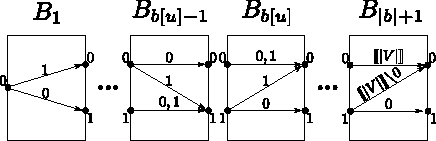
\includegraphics[]{IJCAI25/Figures/OBDDsResized/IntroInput.pdf}
    \caption{Input OBDD $\ODD$}
    \label{fig:IntroInput}
\end{figure}

\begin{figure}[H]
    \centering
    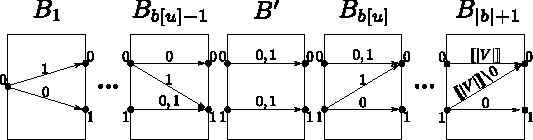
\includegraphics[width=1\linewidth]{IJCAI25/Figures/OBDDsResized/InVrt.pdf}
    \caption{$\symbintrovertex{\activelabelu}(\activelabels, \ODD)$}
    \label{fig:InVrt}
\end{figure}

We define layer $\B'$ to have $|\Dom(\B_{\activelabels[\activelabelu]})|$ many left and right states, and two transitions labeled $0$ and $1$ respectively between each pair of states from $\Dom(\B')$ and $\im(\B')$ with matching indices. Formally, $\B' = \{(i,l,i):l \in \dbset{2}, i \in \Dom(\B_{\activelabels[\activelabelu]})\}$.

\subsection{Intro Edge}\label{section:IntroEdge}

In the standard DP-core for {\sc Vertex Cover} (Appendix \ref{subsection:VC}, Definition \ref{VCDP-core}), if $w$ is a local witness corresponding to a node $p$ with set of active labels $b$, then when introducing an edge $\{u,v\}$, the witness $w$ is added to the newly created set of local witnesses if and only if $w$ takes value $1$ at index $\activelabels[\activelabelu]$ or $\activelabels[\activelabelv]$. Consequently, for OBDD $\ODD$ representing a witness set, symbolic operation $\symbintroedge{\activelabelu}{\activelabelv}(\activelabels, \ODD) = \ODD \cap \ODD^{\{\activelabelu,\activelabelv\}}$ outputs the intersection of $\ODD$ and OBDD $\ODD^{\{\activelabelu,\activelabelv\}}$ of size $|\ODD|$ accepting all binary strings taking value $1$ in at least one of indices $\activelabels[\activelabelu]$ and $\activelabels[\activelabelv]$.

OBDD $\ODD^{\{\activelabelu,\activelabelv\}}$ is illustrated in Figure \ref{fig:IntroedgeODD} below.

\begin{figure}[h]
    \centering
    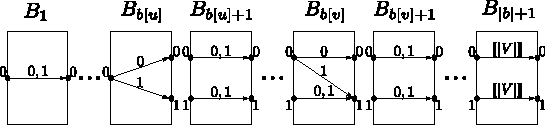
\includegraphics[width=1\linewidth]{IJCAI25/Figures/OBDDsResized/InEdg.pdf}
    \caption{OBDD $\ODD^{\{\activelabelu,\activelabelv\}}$}
    \label{fig:IntroedgeODD}
\end{figure}

In other words, OBDD $\ODD^{\{\activelabelu,\activelabelv\}}$ accepts any length $|\activelabels|+1$ string under our alphabet, provided its value at entries $\activelabels[\activelabelu]$ and $\activelabels[\activelabelv]$ are not both $0$. The intersection $\ODD \cap \ODD^{\{\activelabelu,\activelabelv\}}$ therefore results in an OBDD accepting all strings accepted by input OBDD $\ODD$, except for strings with value $0$ at both entries $\activelabels[\activelabelu]$ and $\activelabels[\activelabelv]$.

We define OBDD $\ODD^{\{\activelabelu,\activelabelv\}} = \B_1\dots \B_{|\activelabels|+1}$ formally as follows. The first $\activelabels[\activelabelu] -1$ layers each consist of a single left state, a single right state, and two transitions labeled $0$ and $1$ respectively; $\B_i = \{(0,0,0), (0,1,0)\}$ for $i \in [\activelabels[\activelabelu] -1]$. At layer $\activelabels[\activelabelu]$, the OBDD forks, with one transition reaching state $0$ upon reading $0$ and another transition reaching state $1$ upon reading $1$; $\B_{\activelabels[\activelabelu]} = \{(0,0,0),(0,1,1)\}$. Subsequent layers up to layer $\activelabels[\activelabelv]-1$ consist of two left states and two right states, with transitions labeled $0$ and $1$ between states with matching indices; $\B_i = \{(0,0,0),(0,1,0),(1,0,1),(1,1,1)\}$ for $i \in \{\activelabels[\activelabelu]+1,\ldots,\activelabels[\activelabelv]-1\}$. At layer $\activelabels[\activelabelv]$, the transitions ensure that strings with $0$ at both positions are rejected. Specifically, layer $\activelabels[\activelabelv]$ contains a transition labeled $0$ form left state indexed $0$ to right state indexed $0$ (witnesses reading $0$ with this transition will go on to be rejected) as well as a transition labeled $1$ from left state labeled $0$ to right state labeled $1$ and transitions labeled $0$ and $1$ from left state labeled $1$ to right state labeled $1$; $\B_{\activelabels[\activelabelv]} = \{(0,0,0),(0,1,1),(1,0,1),(1,1,1)\}$.
Subsequent layers up to the $|\activelabels|$-th again consist of two left states and two right states, with transitions labeled $0$ and $1$ between states with matching indices; $\B_i = \{(0,0,0),(0,1,0),(1,0,1),(1,1,1)\}$. Finally, the $|\activelabels|+1$-th layer consists of two left states and a transition labeled $i$ for each $i\in \dbset{|V|}$ from left state indexed $0$ to the reject state, and left state indexed $1$ to the accept state.

\subsection{Forget Vertex}

In the standard DP-core for {\sc Vertex Cover} (Appendix \ref{subsection:VC}, Definition \ref{VCDP-core}), if $w$ is a local witness corresponding to a node $p$ with set of active labels $b$, when forgetting a label $u$, then $w$ gives rise to a single local witness which corresponds to removing label $u$ from the set component of $w$. Additionally in this case the size of the witness is incremented by 1. At this point in time, the size component counts all vertices that belong to a partial solution and that have been forgotten so far. To simulate this with symbolic operations on an input OBDD $\ODD = B_1\ldots B_{|\activelabels|+1}$ representing a witness set, we first compute the union of intermediate OBDDs $\ODD^{\activelabels[\activelabelu]=0} $ and $\ODD^{\activelabels[\activelabelu]=1}$ where both these OBDDs are modifications of the input OBDD $\ODD$.

Intermediate OBDD $\ODD^{\activelabels[\activelabelu]=0}$ only accepts strings that are accepted by OBDD $\ODD$ and take value $0$ at position $\activelabels[\activelabelu]$. These are witness strings for which the size of the solution they represent need not be incremented upon application of operation $\forgetvertex{\activelabelu}$. Figure \ref{fig:forgetvertexD'} below shows an example of the construction of OBDD $\ODD^{\activelabels[\activelabelu]=0}$ from a given input OBDD $\ODD$ (figure \ref{fig:frgInput}).

\begin{figure}[H]
    \centering
    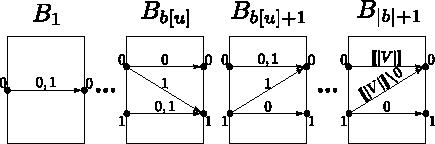
\includegraphics[width=1\linewidth]{IJCAI25/Figures/OBDDsResized/FrgInput.pdf}
    \caption{Input OBDD $\ODD$ }
    \label{fig:frgInput}
\end{figure}

\begin{figure}[H]
    \centering
    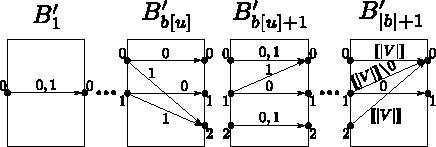
\includegraphics[width=1\linewidth]{IJCAI25/Figures/OBDDsResized/Frgbu0.pdf}
    \caption{Intermediate OBDD $\ODD^{\activelabels[\activelabelu]=0}$}
    \label{fig:forgetvertexD'}
\end{figure}

The layers of $\ODD^{\activelabels[\activelabelu]=0} = B_1'\ldots B_{|b|+1}'$ are defined formally as follows. The first $\activelabels[\activelabelu]-1$ layers are identical to those of the input OBDD; that is, $B_i' = B_i$ for $i \in [\activelabels[\activelabelu]-1]$. At layer $\activelabels[\activelabelu]$, we modify $B_{\activelabels[\activelabelu]}$ to obtain $B_{\activelabels[\activelabelu]}'$ by removing all transitions labeled $1$ and redirecting them to a new right state. Specifically, we define $B_{\activelabels[\activelabelu]}' = (B_{\activelabels[\activelabelu]} \setminus B_{\activelabels[\activelabelu]}^-)\cup B_{\activelabels[\activelabelu]}^+$, where $B_{\activelabels[\activelabelu]}^- = \{(i,1,j) \in B_{\activelabels[\activelabelu]}\}$ and $B_{\activelabels[\activelabelu]}^+ = \{(i,1,|\im(B_{\activelabels[\activelabelu]})|) : i \in \Dom(B_{\activelabels[\activelabelu]})\}$.  This modification ensures that strings reading $1$ at layer $\activelabels[\activelabelu]$ will go on to be rejected.

For each subsequent layers $i$ from $\activelabels[\activelabelu]+1$ to $|\activelabels|$, we add a new left state and a new right state to the layer, including transitions labeled $0$ and $1$ between these new states. Formally, $B_i' = B_i \cup \{(|\Dom(B_i)|,l,|\im(B_i)|): l \in \{0,1\}\}$. At the final layer $B_{|\activelabels|+1}$, we add transitions from the new left state to the reject state labeled with all possible sizes $l \in [|V|]$, defining $B_{|\activelabels|+1}'= B_{|\activelabels|+1}\cup\{(|\Dom(B_{|\activelabels|+1})|,l,r): l \in [|V|]\}$.

On the other hand, intermediate OBDD $\ODD^{\activelabels[\activelabelu]=1}$ is a modification of input OBDD $\ODD$ that only accepts strings accepted by $\ODD$ which take value $1$ at entry $\activelabels[\activelabelu]$. These are witness strings for which the size of the solution they represent are incremented upon application of operation $\forgetvertex{\activelabelu}$. The figure below shows an example of the construction of OBDD $\ODD^{\activelabels[\activelabelu]=1}$ from input OBDD $\ODD$ (figure \ref{fig:frgInput}).

\begin{figure}[h]
    \centering
    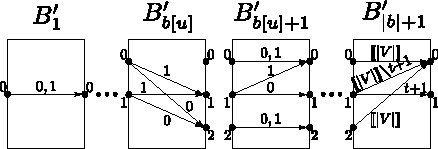
\includegraphics[width=1\linewidth]{IJCAI25/Figures/OBDDsResized/frgbu1.pdf}
    \caption{OBDD $\ODD^{\activelabels[\activelabelu]=1}$}
    \label{fig:forgetvertexD''}
\end{figure}

The layers of $\ODD^{\activelabels[\activelabelu]=1}= B_1'\ldots B_{|b|+1}'$ are defined as follows. The first $\activelabels[\activelabelu]-1$ layers remain the same as in $\ODD$; that is, $B_i' = B_i$ for $i \in [\activelabels[\activelabelu]-1]$. At layer $\activelabels[\activelabelu]$, we construct $B_{\activelabels[\activelabelu]}'$ by including all transitions labeled $1$ from the original layer, forming $B_{\activelabels[\activelabelu]}^* = \{(i,1,j) \in B_{\activelabels[\activelabelu]}\}$, and redirecting all transitions labeled $0$ to a new right state, forming $B_{\activelabels[\activelabelu]}^+ = \{(i,0,|\im(B_{\activelabels[\activelabelu]})|): i \in \Dom(B_{\activelabels[\activelabelu]})\}$. Thus, $B_{\activelabels[\activelabelu]}' = B_{\activelabels[\activelabelu]}^* \cup B_{\activelabels[\activelabelu]}^+$.

For layers $\activelabels[\activelabelu]+1$ to $|\activelabels|$, we again add a new left state and a new right state, including transitions labeled $0$ and $1$ between them: $B_i' = B_i \cup \{(|\Dom(B_i)|, l, |\im(B_i)|): l \in \{0,1\}\}$. At the final layer, we adjust the labels of the transitions by incrementing the size component by $1$ to account for the increment in the size of partial solutions when the value at position $\activelabels[\activelabelu]$ is $1$. Specifically, we define $B_{|\activelabels|+1}' = B_{|\activelabels|+1}^* \cup \{(|\Dom(B_{|\activelabels|+1})|, l, r): l \in [n]\}$, where $B_{|\activelabels|+1}^* = \{(i, l+1, a): (i, l, a) \in B_{|\activelabels|+1}\}$.

The union of OBDDs $\ODD^{\activelabels[\activelabelu]=0}$ and $\ODD^{\activelabels[\activelabelu]=1}$ is an OBDD where the size component of witnesses is accounted for with respect to label $\activelabelu$. Finally, we remove layer $B_{\activelabels[\activelabelu]}$ from $\ODD^{\activelabels[\activelabelu]=0} \cup \ODD^{\activelabels[\activelabelu]=1} = B_1\ldots B_{\activelabels[\activelabelu]-1}B_{\activelabels[\activelabelu]}\ldots B_{|\activelabels|+1}$ to create output OBDD $\ODD^* = B_1\ldots B^*_{\activelabels[\activelabelu]-1}\ldots B_{|\activelabels|+1}$, where layer $B^*_{\activelabels[\activelabelu]-1}$ is a modification of layer $B_{\activelabels[\activelabelu]-1}$ formally denoted $B^*_{\activelabels[\activelabelu]-1} = \{(i,l,j): (i,l,h)\in B_{\activelabels[\activelabelu]-1}, (h,l',j)\in B_{\activelabels[\activelabelu]}\}$. This replaces the right states of $B_{\activelabels[\activelabelu]-1}$ with right states of $B_{\activelabels[\activelabelu]}$ and creates a transition $(i,l,j)$ if it was possible to reach right state $j$ of layer $B_{\activelabels[\activelabelu]}$ after reading a transition labeled $l$ in $B_{\activelabels[\activelabelu]-1}$. This ensures that witnesses contracted at position $\activelabels[\activelabelu]$ go on to be appropriately accepted (rejected).
An example of the transformation from $\ODD^{\activelabels[\activelabelu]=0} \cup \ODD^{\activelabels[\activelabelu]=1}$ to $\ODD^*$ is shown in the figure below:

\begin{figure}[h]
    \centering
    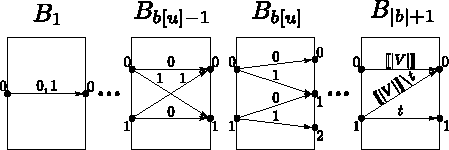
\includegraphics[width=1\linewidth]{IJCAI25/Figures/OBDDsResized/FrgCap.pdf}
    \caption{OBDD $\ODD^{\activelabels[\activelabelu]=0} \cup \ODD^{\activelabels[\activelabelu]=1}$}
    \label{fig:frgCap}
\end{figure}


\begin{figure}[h]
    \centering
    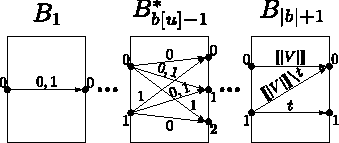
\includegraphics[width=1\linewidth]{IJCAI25/Figures/OBDDsResized/FrgVrt.pdf}
    \caption{OBDD $\ODD^*=\symbforgetvertex{\activelabelu}(b,\ODD)$}
    \label{fig:forgetvertexDstar}
\end{figure}

\subsection{Join}

In the standard DP-core for {\sc vertex cover} (Appendix \ref{subsection:VC}, Definition \ref{VCDP-core}), if $w$ is a local witness corresponding to a node $p$ with set of active labels $b$, the join operation takes two local wintesses $w_1$ and $w_2$ and produces a local witness $w$ that has the same set component as $w_1$ and $w_2$, but where the size component $t$ is the sum of the size components $t_1$ and $t_2$ of $w_1$ and $w_2$ respectively. 

To reflect this, operation $\symbjoin(\ODD_1,\ODD_2) $ produces an OBDD accepting only witnesses from both $\ODD_1$ and $\ODD_2$ with aggregated sizes components. Note that OBDD $\ODD_1 \cup \ODD_2$ upon minimization yields and OBDD where witnesses $st_1$ and $st_2$ with like string components follow an identical sequence of transitions up to left state $i$ of the last layer. From here, transitions $(i,t_1,a)$ and $(i,t_2,a)$ accepts witnesses $st_1$ and $st_2$ respectively. Leveraging this observation, at each left state of the final layer we could identify pairs of transitions leading to the accept state and replace them with a single transition with summed label. This strategy however would not capture witnesses pairs with identical string and size components.
Therefore we instead compute the union of intermediate OBDDs $\ODD^{\scriptcap}$ and $\ODD^{\scriptcup}$. The OBDD $\ODD^{\scriptcap}$ is a modification of the intersection $\ODD_1 \cap \ODD_2$ of the input OBDDs. Note that $\ODD_1 \cap \ODD_2 = B_1\ldots B_{|\activelabels|+1}$ is an OBDD accepting only witnesses present in both $\Lang(\ODD_1)$ and $\Lang(\ODD_2)$ with identical string component and size. We modify this OBDD at its final layer to correctly reflect the $\join$ operation on these witnesses by doubling the sizes for witnesses read in the final layer. Specifically, we define OBDD $\ODD^{\scriptcap} = B_1^{\scriptcap}\ldots B_{|\activelabels|+1}^{\scriptcap}$, where for $i \in [|\activelabels|]$, $B_i^{\scriptcap} = B_i$, and at the final layer, $B_{|\activelabels|+1}^{\scriptcap} = B_{|\activelabels|+1}^a \cup B_{|\activelabels|+1}^r$, where $B_{|\activelabels|+1}^a = \{(i,2 \cdot l,a): (i,l,a)\in B_{|\activelabels|+1}\}$ and $B_{|\activelabels|+1}^r = \{(i,l,r): (i,l,r)\in B_{|\activelabels|+1}\}$. 

Next, we compute the OBDD $\ODD^{\scriptcup}$, a modification of the OBDD $\ODD_1 \cup \ODD_2= B_1\ldots B_{|\activelabels|+1}$. While the union of OBDDs $\ODD_1$ and $\ODD_2$ would accept any witnesses read by either OBDD, we modify the transitions in the final layer to ensure that only witnesses present in both $\ODD_1$ and $\ODD_2$ are accepted, with their size components summed accordingly. 
For layers $i \in [|\activelabels|]$, we have $B_i^{\scriptcup} = B_i$. At the final layer, we define $B_{|\activelabels|+1}^{\scriptcup}$ as the union of two sets: $B_{|\activelabels|+1}^a$ and $B_{|\activelabels|+1}^r$. The set $B_{|\activelabels|+1}^a$ consists of transitions from left state $i$ to the accept state $a$, labeled with the sum $x + y$, where there exist transitions $(i,x,a)$ and $(i,y,a)$ in $B_{|\activelabels|+1}$ with $x \neq y$. Formally, $B_{|\activelabels|+1}^a = \{(i,x + y,a): (i,x,a),(i,y,a)\in B_{|\activelabels|+1}, x\neq y\}$. The set $B_{|\activelabels|+1}^r$ consists of transitions from left state $i$ to the reject state $r$, labeled with sizes $x \in [|V|]$ such that there is no corresponding pair of transitions to form a sum in $B_{|\activelabels|+1}^a$. Formally, $B_{|\activelabels|+1}^r = \{(i,x,r): i \in \Dom(B_{|\activelabels|+1}), x \in [|V|], (i,x,a) \notin B_{|\activelabels|+1}^a\}$.

%Finally, we let the output OBDD $\ODD^* = \ODD^{\scriptcap} \cup \ODD^{\scriptcup} = \symbjoin$ be the union of our two intermediate OBDDs.
